\documentclass[12pt,letterpaper]{article}
\usepackage{graphicx,textcomp}
\usepackage{natbib}
\usepackage{setspace}
\usepackage{fullpage}
\usepackage{color}
\usepackage[reqno]{amsmath}
\usepackage{amsthm}
\usepackage{fancyvrb}
\usepackage{amssymb,enumerate}
\usepackage[all]{xy}
\usepackage{endnotes}
\usepackage{lscape}
\newtheorem{com}{Comment}
\usepackage{float}
\usepackage{hyperref}
\newtheorem{lem} {Lemma}
\newtheorem{prop}{Proposition}
\newtheorem{thm}{Theorem}
\newtheorem{defn}{Definition}
\newtheorem{cor}{Corollary}
\newtheorem{obs}{Observation}
\usepackage[compact]{titlesec}
\usepackage{dcolumn}
\usepackage{tikz}
\usetikzlibrary{arrows}
\usepackage{multirow}
\usepackage{xcolor}
\newcolumntype{.}{D{.}{.}{-1}}
\newcolumntype{d}[1]{D{.}{.}{#1}}
\definecolor{light-gray}{gray}{0.65}
\usepackage{url}
\usepackage{listings}
\usepackage{color}

\definecolor{codegreen}{rgb}{0,0.6,0}
\definecolor{codegray}{rgb}{0.5,0.5,0.5}
\definecolor{codepurple}{rgb}{0.58,0,0.82}
\definecolor{backcolour}{rgb}{0.95,0.95,0.92}

\lstdefinestyle{mystyle}{
	backgroundcolor=\color{backcolour},   
	commentstyle=\color{codegreen},
	keywordstyle=\color{magenta},
	numberstyle=\tiny\color{codegray},
	stringstyle=\color{codepurple},
	basicstyle=\footnotesize,
	breakatwhitespace=false,         
	breaklines=true,                 
	captionpos=b,                    
	keepspaces=true,                 
	numbers=left,                    
	numbersep=5pt,                  
	showspaces=false,                
	showstringspaces=false,
	showtabs=false,                  
	tabsize=2
}
\lstset{style=mystyle}
\newcommand{\Sref}[1]{Section~\ref{#1}}
\newtheorem{hyp}{Hypothesis}

\title{Problem Set 2}
\date{Due: October 14, 2024}
\author{Applied Stats/Quant Methods 1}

\begin{document}
	\maketitle
	\section*{Instructions}
\begin{itemize}
	\item Please show your work! You may lose points by simply writing in the answer. If the problem requires you to execute commands in \texttt{R}, please include the code you used to get your answers. Please also include the \texttt{.R} file that contains your code. If you are not sure if work needs to be shown for a particular problem, please ask.
	\item Your homework should be submitted electronically on GitHub.
	\item This problem set is due before 23:59 on Monday October 14, 2024. No late assignments will be accepted.

\end{itemize}

	
	\vspace{.5cm}
	\section*{Question 1: Political Science}
		\vspace{.25cm}
	The following table was created using the data from a study run in a major Latin American city.\footnote{Fried, Lagunes, and Venkataramani (2010). ``Corruption and Inequality at the Crossroad: A Multimethod Study of Bribery and Discrimination in Latin America. \textit{Latin American Research Review}. 45 (1): 76-97.} As part of the experimental treatment in the study, one employee of the research team was chosen to make illegal left turns across traffic to draw the attention of the police officers on shift. Two employee drivers were upper class, two were lower class drivers, and the identity of the driver was randomly assigned per encounter. The researchers were interested in whether officers were more or less likely to solicit a bribe from drivers depending on their class (officers use phrases like, ``We can solve this the easy way'' to draw a bribe). The table below shows the resulting data.

\newpage
\begin{table}[h!]
	\centering
	\begin{tabular}{l | c c c }
		& Not Stopped & Bribe requested & Stopped/given warning \\
		\\[-1.8ex] 
		\hline \\[-1.8ex]
		Upper class & 14 & 6 & 7 \\
		Lower class & 7 & 7 & 1 \\
		\hline
	\end{tabular}
\end{table}

\begin{enumerate}
	
	\item [(a)]
	Calculate the $\chi^2$ test statistic by hand/manually (even better if you can do "by hand" in \texttt{R}).\\
	
	There are 5 steps I will follow in order to calculate the Chi-squre test statistic.\\ 
		\vspace{.05cm}\\
\textbf{Step 1: Set up the Null}\\

$H_0$: There is no association between the social class of the driver and whether police offers would solicit a  bribe.\\
$H_a$: There is an association between the social class of the driver and whether police offers would solicit a  bribe.\\

From here, I am going to calculate a test-statistic (the $X^2$ statistic) that is distributed according to the $X^2$ distribution.

The $F_0$ tells us the observed frequency and $F_e$ tells us what we should expect were the samples independent (if there were no relationship between class and solicited bribes)

This requires the following equation calculates the $X^2$ statistic:
\begin{center}
$\chi^2 = \sum \frac{(f_0 - f_e)^2}{f_e}$
\end{center}


\textbf{Step 2: Construct Contingency Table}\\ 

I will construct the contingency table which requires adding the totals from each row and column. The values in each cell tell is the observed frequency. We do this because the rows and collums represent different values of interest. The collums in this case show different oucomes but for this analysis, we care about these outcomes equally. The rows tell us class levels but, again, for the time being we care about class generally. 

\textbf{Step 3: Calculate the Expected Frequencies}\\ 

We now need to calculate the expected frequencies for each cell. This is done using the forementioned equation only applied to each individual cell within the contingency table. The sum of each of these, provides us with the  $X^2$ statistic of interested. 

To calculate the $F_e$ of the first cell (the "Not Stopped" "Upper Class" with an $F_0$ of 14), we apply the equation in the following way:\\ 
\begin{center}
$F_e{1} = \frac{(27 \times 21)}{42} = \frac{567}{42} = 13.5$
\end{center}

This process is repeated for every square in order to get the expected frequency of each. Once we have the contingency table completed showing the expected frequency of each square, we are ready to then caluclate the chi-square statistic. 

\textbf{Step 4: Compute the Chi-square Statistic}\\

Now we want to calculate the  $X^2$ statistic. This is done by taking the observed frequency minus substracting the expected frquency, squared. This figure is then divided by the expected frequency of the cell. This is repeated for each cell within the contingency table and, finally, they are added. The equation is the aforementioned. The example below, shows how I calculate the first cell from the contingency table (Upper Class, Not Stopped)
\begin{center}
$\frac{(14 - 13.5)^2}{13.5} = \frac{0.25}{13.5} = 0.0185$
\end{center}

According to R, our overall $X^2$ statistic of interest is approcimately \textbf{3.791}. 

\textbf{Step 5: Determine the Degrees of Freedom}\\

To calculate the degrees of freedom, we use the following equation:\\ 
\begin{center}
$\text{df} = (\text{rows} - 1)(\text{columns} - 1)$\\

$\text{df} = (2 - 1) \times (3 - 1) = 1 \times 2 = 2$
\end{center}

In this case, there are two rows and 3 collums, so we have two degrees of freedom. 

\textbf{Step 6: Conclusion: Compare Chi Square with Critical Value.}

The critical value here for 0.05, corresponding to two degrees of freedom is approcimately \textbf{5.991}. Given that our overall $X^2$ statistic of interest is approximately \textbf{3.791}, it is lower than our critical value. \textbf{This means that we cannot reject $H_0$.}  

	\vspace{7cm}
	\item [(b)]
	Now calculate the p-value from the test statistic you just created (in \texttt{R}).\footnote{Remember frequency should be $>$ 5 for all cells, but let's calculate the p-value here anyway.}  What do you conclude if $\alpha = 0.1$?\\

The p-value for the chi-square test statistic of \textbf{3.791} with \textbf{2} degrees of freedom is approximately \textbf{0.150}
Since the p-value (0.150) is greater than the significance level \textbf{$\alpha = 0.1$}, we do \textbf{not} reject the null.

	\item [(c)] Calculate the standardized residuals for each cell and put them in the table below.
	\vspace{1cm}

The standardised residuals tell us how far away each observed value is from the "expectation". We need to calculate the adjusted residual for each square and do this using the following calculation: 
\[
z = \frac{f_{\text{observed}} - f_{\text{expected}}}{\text{se}}
\]

\[
\text{se} = \sqrt{f_{\text{expected}} \cdot (1 - \text{row proportion}) \cdot (1 - \text{column proportion})}
\]

According to R, the standardised residuals are as follows: 

\begin{table}[h]
	\centering
	\begin{tabular}{l | c c c }
		& Not Stopped & Bribe requested & Stopped/given warning \\
		\\[-1.8ex] 
		\hline \\[-1.8ex]
		Upper class  & 0.1360828 & -0.8153742 & 0.818923\\
		\\
		Lower class & -0.1825742 & 1.0939393 & -1.098701 \\
		
	\end{tabular}
\end{table}
	
	\item [(d)] How might the standardized residuals help you interpret the results?  


The standardised residuals, as shown in the table above, tell us how far away each observed value is from the expectation. Taking the first cell as an example, we can sat that the 'Not stopped' 'Upper Class' is approcimately 0.14 which means that it is close to the expected value. The positive residuals in the table tell us that the observed frequency is higher than expected, and the negative residuals tell us that the observed frequency is lower than expected. For example, bribes for the 'Upper Class' were requested will lesser frequency (-1.82) than we would expect.\\

 
The R Code is included on the following page 

\newpage
\lstinputlisting[language=R, firstline=1, lastline=43]{Problem Set 2 JM.R}  

\end{enumerate}
\newpage

\section*{Question 2: Economics}
Chattopadhyay and Duflo were interested in whether women promote different policies than men.\footnote{Chattopadhyay and Duflo. (2004). ``Women as Policy Makers: Evidence from a Randomized Policy Experiment in India. \textit{Econometrica}. 72 (5), 1409-1443.} Answering this question with observational data is pretty difficult due to potential confounding problems (e.g. the districts that choose female politicians are likely to systematically differ in other aspects too). Hence, they exploit a randomized policy experiment in India, where since the mid-1990s, $\frac{1}{3}$ of village council heads have been randomly reserved for women. A subset of the data from West Bengal can be found at the following link: \url{https://raw.githubusercontent.com/kosukeimai/qss/master/PREDICTION/women.csv}\\

\noindent Each observation in the data set represents a village and there are two villages associated with one GP (i.e. a level of government is called "GP"). Figure~\ref{fig:women_desc} below shows the names and descriptions of the variables in the dataset. The authors hypothesize that female politicians are more likely to support policies female voters want. Researchers found that more women complain about the quality of drinking water than men. You need to estimate the effect of the reservation policy on the number of new or repaired drinking water facilities in the villages.


\vspace{.5cm}
\begin{figure}[h!]
	\caption{\footnotesize{Names and description of variables from Chattopadhyay and Duflo (2004).}}
	\vspace{.5cm}
	\centering
	\label{fig:women_desc}
	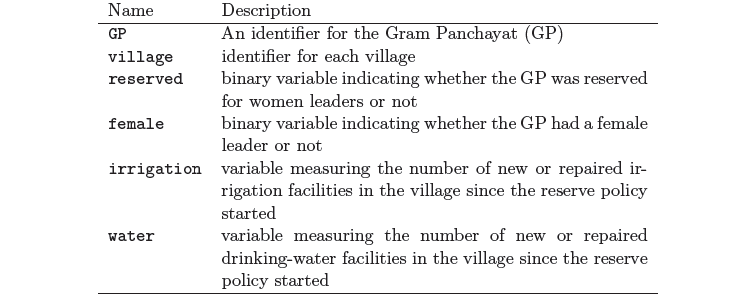
\includegraphics[width=1.1\textwidth]{women_desc.png}
\end{figure}		

\newpage
\begin{enumerate}
	\item [(a)] State a null and alternative (two-tailed) hypothesis.\\
	 
$\textbf{Null Hypothesis (} H_0 \textbf{):}$ \\
	\text{The coucil's female reservation policy doesn't have an effect on the number of new or repaired drinking water facilities in the villages.} \\
$H_0: \beta_1 = 0$\\
	
$\textbf{Alternative Hypothesis (} H_a \textbf{):}$ \\
\text{The council's female reservation policy has an effect on the number of new or repaired drinking water facilities in the villages.} \\
$H_0: \beta_1 = 0$	
	\vspace{1cm}
	\item [(b)] Run a bivariate regression to test this hypothesis in \texttt{R} (include your code!).
\begin{table}[!htbp] \centering 
	\caption{} 
	\label{} 
	\begin{tabular}{@{\extracolsep{5pt}}lc} 
		\\[-1.8ex]\hline 
		\hline \\[-1.8ex] 
		& \multicolumn{1}{c}{\textit{Dependent variable:}} \\ 
		\cline{2-2} 
		\\[-1.8ex] & water \\ 
		\hline \\[-1.8ex] 
		reserved & 9.252$^{**}$ \\ 
		& (3.948) \\ 
		& \\ 
		Constant & 14.738$^{***}$ \\ 
		& (2.286) \\ 
		& \\ 
		\hline \\[-1.8ex] 
		Observations & 322 \\ 
		R$^{2}$ & 0.017 \\ 
		Adjusted R$^{2}$ & 0.014 \\ 
		Residual Std. Error & 33.446 (df = 320) \\ 
		F Statistic & 5.493$^{**}$ (df = 1; 320) \\ 
		\hline 
		\hline \\[-1.8ex] 
		\textit{Note:}  & \multicolumn{1}{r}{$^{*}$p$<$0.1; $^{**}$p$<$0.05; $^{***}$p$<$0.01} \\ 
	\end{tabular} 
\end{table} 


	\vspace{1cm}
	\item [(c)] Interpret the coefficient estimate for reservation policy. 
	
The 'reserved' coefficient estimate is \textbf{9.252.} This means that villages in which the council have position's reserved for women also have, on average, 9.252 more new or repaired drinking water facilities in the villages. Furthermore, the p-value for this coefficient is \textbf{0.0197*}, which is less than the level of statistical significance at 0.05. We therefore have evidence that indicates that the effect of the council's female reservation policy on the number of drinking water facilities is statistically significant. Consequently, we can reject the null hypothesis. 
\end{enumerate}
\lstinputlisting[language=R, firstline=46, lastline=62]{Problem Set 2 JM.R}  
\end{document}
